%% It is just an empty TeX file.
%% Write your code here.
\chapter{Communication System Test}\label{ch:experiment}

\section{Functional Shorts Implementation}
To verify the functional test concept an example communication system has been built and shown in \autoref{fig:short_ena}. The implementation lacks real modules, except from the encoder and decoder. Every other module is implemented as a simple delay in the digital information flow (flip flop) and XOR gate to conduct the error injection. They also have special enable signal to choose which module should occur as faulty. The AIR simulates the communication channel. There is also a programmable delay to variate the execution time of the test and to simulate the fact, that the number of clock cycles, needed for the information to pass from the encoder to decoder, is not constant in all tests. The short enable signals control the data flow in the test loop. The activation of any short, excludes the whole part of the system laying beyond the short and shortens the test duration, because the information doesn't need to be clocked through all excluded modules. The injected error vector travels through the design together with the test data. This guaranties the proper alignment of the error vector with the test vector at any time, also during the shortcut, when the path is shorter. The error vector flips the specified bits of the output of any chosen module to simulate the possible effects of hardware faults on the processed information. The error enable signal is exclusive, meaning that only one module may be faulty at the same time. 

\begin{figure}[h]
\centering
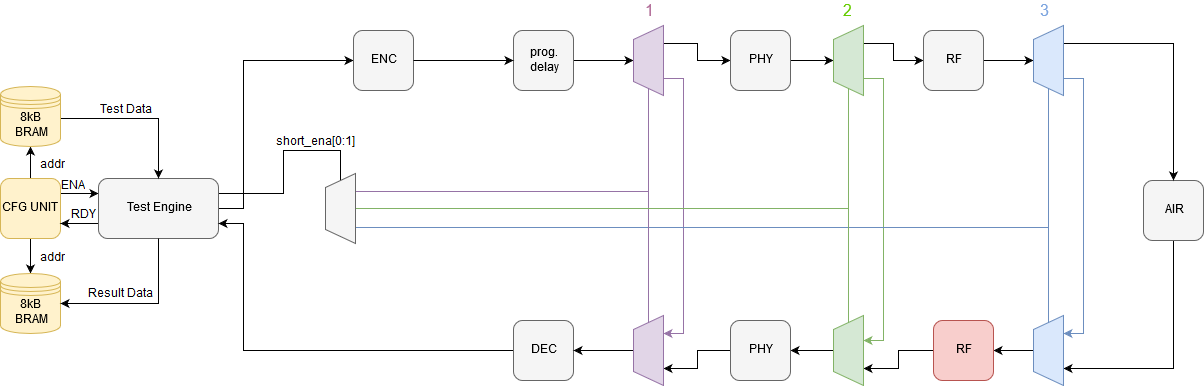
\includegraphics[width=\textwidth]{figures/Short_ena_err.png}
\caption{Implementation of functional shorts into the Test Bench}
\label{fig:short_ena}
\end{figure}

The experimental set-up has been implemented into the Test Bench. It consists of the BCH(1023,943) Encoder and Decoder, being able to correct up to 8 bit errors. The encoder and decoder need a reset signal to start working. The reset is followed by 943 random data bits and 80 zeros to compute the parity bits in the encoder. Parallel to these 1023 encoder bits, a 1023 bit error vector is shifted in. The bit that is supposed to be flipped is set to one, the rest to zero. The data block and the error vector are appended by the zero vector of the following length. The size of the programmable delay plus one for every module in the current test loop. The excluded modules laying beyond the active short, are not counted. The decoder needs additional 97 clock cycles for syndrome calculations and error localization, therefore another 97 zeros need to be added to the input signals. To shift out the corrected user bits another 943 cycles are needed. To monitor the error detection in the whole block, another 80 bits can be shifted out. The decoder response lies in the last 1023 bits of the output bitstream, so do 1023 special output bits, indicating the correction.

All tests revealed, that the method can be used for systematic fault diagnosis on the module level. Systematic exclusion of modules and test repetition allowed to localize a faulty module in all cases. The number of errors was lower or equal to the correction capability of the decoder. But how do the system react to the higher number of errors and what real errors occur as result of real permanent faults? Firstly the BCH encoder was tested for errors resulting from delay faults. Then fault injection was conducted to observe how the encoder reacts in presence of transient and permanent faults. Then the decoder was tested for error detection above its maximal correction capability and also for delay faults.

\section{Test of BCH(1023,943) Encoder}
The tested encoder is a BCH encoder taking 943 payload bits and calculating 80 parity bits. The encoder is actually a part of the PENCA architecture, without any redundant test and configuration circuitry. The encoder consists of an LFSR for parity calculations and the counter to keep track on the number of input user bits. Before the counter reaches 943 bits, it forwards the user bits to the output and enables linear feedback in the shift register. Then the parities are shifted out with "dummy" input bits with the LFSR acting as simple shift register. The parity calculation is obtained by dividing the input polynomial by the generator polynomial of the encoder. The reminder of the division is the parity polynomial. The general architecture of a BCH encoder using a LFSR for polynomial division is shown in \autoref{fig:enc_0}. Since the test bench developed during the project allows a test with wide range of frequencies, it may be possible to cause some delay faults in the encoder architecture and examine, how they influence the output bit stream.

\begin{figure}[h]
\centering
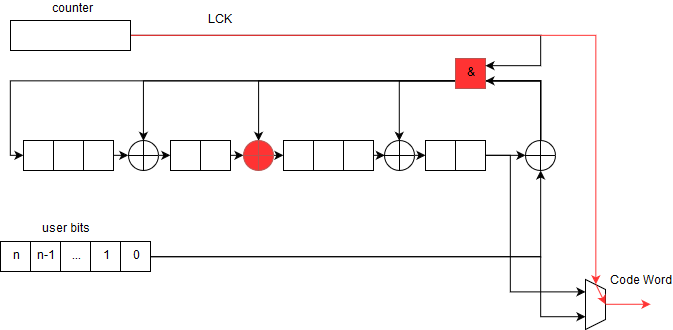
\includegraphics[width=0.65\textwidth]{figures/BCH_ENC.png}
\caption{A BCH encoder architecture \cite{art:BCH_implement}}
\label{fig:enc_0}
\end{figure}

The encoder has been placed in the test bench and tested for maximum frequency. The input data is random. There were 300 messages sent and evaluated. The comparison data was calculated using MATLAB 2015b comm.BCHEncoder. There were two encoder versions tested. One version is surrounded by flip-flops to guarantee that the delay fault happens in the encoder design and not due to the long connection paths between encoder design and the Test Engine. This version was called "isolated". The "not isolated" one was connected simply to the input and output registers of the Test Engine. First clock cycle is reserved for the reset. When the reset is low, the input vector is shifted in serially. The output is equal to the input when the payload bits are shifted in. After 943 payload bits, the input is set to zero and held that way till the end of the test, which means another 80 clock cycles for the parity bits to be shifted out. The test fails when the output value is different from the pre-calcualted value. The frequency is raised until first tests start to fail. This marks the cut-off frequency of the Encoder and reveals the errors caused by delay fault. The cut-off frequencies are presented in \autoref{tab:enc}.

\begin{table}[h]
\begin{tabular}{@{}lllll@{}}
\toprule
UUT                       &mem\_width   &uut\_width &expected freq. &max. freq.\\ 
\midrule
isolated Encoder                  & 32          & 4      & $\sim$642 MHz & $\sim$500 MHz \\
not isolated Encoder              & 32          & 4      & $\sim$642 MHz & $\sim$326 MHz \\
\bottomrule
\end{tabular}
\centering
\caption{Test Encoder for max. frequency}\label{tab:enc}
\end{table}

The result shows clearly, that a Test Engine limit of 500 MHz has been reached while testing the isolated Encoder, the frequency was not raised above this value, because the result would not be reliable. The not-isolated version on the other hand, failed by the frequency of 326 MHz. Both versions differ only in flip-flops isolating them from the test bench, therefore any errors happening in the not-isolated version did not arise in the Encoder itself. They originate from the long connections between the Encoder and the Test Bench. But such errors could also arise due to delay faults in real hardware. 

\autoref{fig:enc_1} represents the result of all failed test of the not-isolated Encoder at approx. 355 MHz. In half of the messages the first parity bit is corrupted. When the counter, calculating the number of shifted bits, reaches the 943, the output should be switched to the parity bits (see \autoref{fig:enc_0}). In all vectors, the output still forwards the input value, which is zero for all "dummy" parity bits. In half of the vectors, since they are randomly distributed, the zero is accidentally the expected value, therefore the error gets masked.

The raised frequency together with very long interconnect simulated a delay fault in the control signal of the multiplexer. The situtation is marked as red line in \autoref{fig:enc_0}. When the counter reaches 943, a special LCK signal is generated to disable feedback in the LFSR and change the source of the output pin to forward LFSR output instead of Encoders input. The outcome is a single bit error in half of the produced code words. This error can be easily detected and corrected by the decoder.

\begin{figure}[h]
\centering
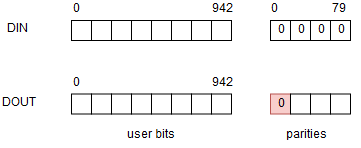
\includegraphics[width=.65\textwidth]{figures/enc_error.png}
\caption{The result of failed Encoder test by 355 MHz}
\label{fig:enc_1}
\end{figure}



\section{Test of BCH(1023,943) Decoder}
For any positive integers $m \geq 3$ and $t<2^{m-1}$ there exists a binary BCH code with the following parameters \cite{art:BCH_implement}:
\begin{subequations}
\begin{align}
    \text{block length }n&=2^{m}-1\label{eq:blck_len}\\
    \text{parity bits }k&\geq n+mt\label{eq:parity}\\
    \text{hamming distance }d&\geq2t+1\label{eq:dmin}
\end{align}
\end{subequations}
The BCH(1023,943) with its $n = 1023$ and $k=943$, has a $d_{min}= 17$. The code is therefore capable of detecting 16 error bits and correcting 8 in a single block. 

The tested BCH decoder has one serial data input (DIN) and one data output (DOUT). The input data enters the syndrome computation block, which is similarly to encoder, implemented as LFSRs. It is actually less complicated then the encoder, having shorter LFSRs to compute partial syndromes, one for every correctable error. When all syndromes are equal zero, the received message is a valid code word. In other case, when any syndrome is non-zero, the Key Equation Solver has to find the parameters of error locating polynomial. The parameters are passed to Chien Search Block to find the roots of the error locating polynomial and therefore the exact positions of errors in the received message. The output of the Chien Search Block is connected to the output ISERR to indicate, if the current output bit has been repaired. This is the special extension allowing the Functional Short Concept to be implemented. The decoder needs 97 clock cycles before it starts shifting out the corrected user bits. The basic idea of building a BCH Decoder is shown in \autoref{fig:dec_0}.

\begin{figure}[h]
\centering
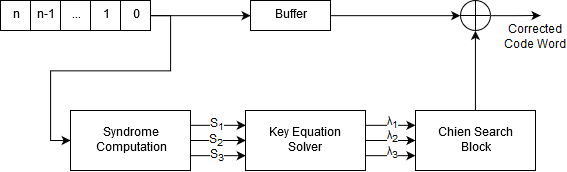
\includegraphics[width=0.65\textwidth]{figures/BCH_DEC.png}
\caption{A BCH decoder architecture \cite{art:BCH_implement}}
\label{fig:dec_0}
\end{figure}

\subsection{Test Decoder for maximal frequency}

The test procedure involving functional shortcuts assumed a fault free functionality of the decoder. It is possible though, that the decoder suffers from any permanent or transient fault itself, giving false negative or false positive results of the test, not mentioning the problems during communication. The decoder was tested for its maximal operational frequency and beyond. The decoder was tested only until its maximal correction capabilities. The isolated version means that the design was surrounded by flip-flops. The direct input and output is always compared with their delayed pairs to check, if the delay fault did not happen on the interface with Test Bench. The unconstrained design allows the tool to automatically place the design in the FPGA. The constrained version forces the tool to place the design closer to the Test Engine. The results are presented in \autoref{tab:dec}.

\begin{table}[h]
\begin{tabular}{@{}ccccll@{}}
\toprule
UUT                       &mem\_width   &uut\_width &error cnt. &\begin{tabular}{@{}c@{}}unconstrained \\max. freq.\end{tabular} &\begin{tabular}{@{}c@{}}constrained \\max. freq.\end{tabular}\\ 
\midrule
\multirow{9}{*}{\begin{tabular}{@{}c@{}}isolated \\Decoder\end{tabular}}    & \multirow{9}{*}{32}        & \multirow{9}{*}{8}       &0           & $\sim$264 MHz & $\sim$319 MHz \\
                            &                           &                           &1          &   $\sim$237 MHz &   $\sim$229 MHz\\
                            &                           &                           &2          &   $\sim$200 MHz &   $\sim$221 MHz\\
                            &                           &                           &3          &   $\sim$200 MHz &   $\sim$219 MHz\\
                            &                           &                           &4          &   $\sim$200 MHz &   $\sim$219 MHz\\
                            &                           &                           &5          &   $\sim$180 MHz &   $\sim$218 MHz\\          
                            &                           &                           &6          &   $\sim$160 MHz &   $\sim$219 MHz\\
                            &                           &                           &7          &   $\sim$160 MHz &   $\sim$218 MHz\\
                            &                           &                           &8          &   $\sim$160 MHz &   $\sim$219 MHz\\
\bottomrule
\end{tabular}
\centering
\caption{Test Decoder for max. frequency}\label{tab:dec}
\end{table}

In the unconstrained version, the routing tool decided to place the isolating registers far away from the decoder and close to the Test Engine. This made the isolation useless and didn't allow to detect the delay faults happening on the interconnects with the Test Engine. Constraining the design was the only way to force the tool to make the isolating registers part of the decoder design. The unconstrained design is presented in \autoref{subfig:uncon}.

\begin{figure}[h]
\centering
\begin{subfigure}{.45\textwidth}
    \centering
    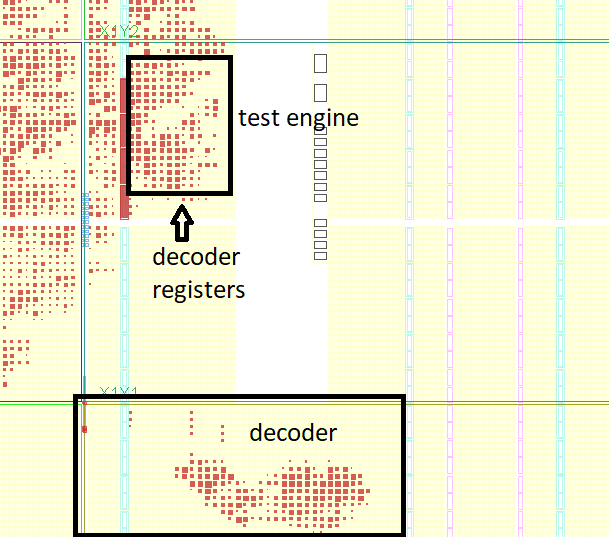
\includegraphics[width=\linewidth]{figures/Device_edited.png}
    \caption{Unconstrained}
    \label{subfig:uncon}
\end{subfigure}%
\hspace{\fill}
\begin{subfigure}{.45\textwidth}
    \centering
    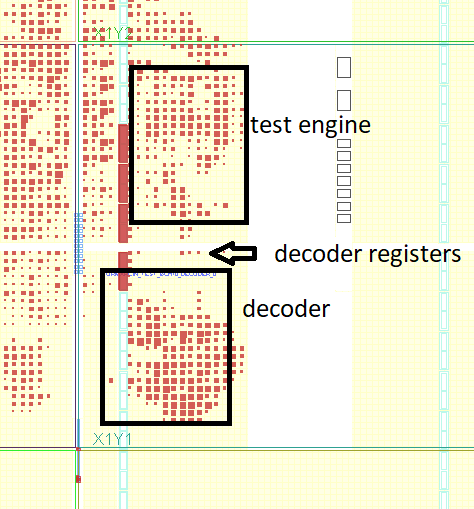
\includegraphics[width=\linewidth]{figures/Device_Pblock_edited.png}
    \caption{Constrained}
    \label{subfig:con}
\end{subfigure}
\caption{Decoder placement in FPGA}
\label{fig:dec_routing}
\end{figure}

Since the design can be influenced by constraining the placement tool, the further tests were conducted on a decoder enclosed in so called PBLOCK. The PBLOCKS are areas in the FPGA, that force the placement tool to try to fit parts of the design inside of them. After drawing the PBLOCK between the old decoder position and the test engine, the decoder was placed closer to the test engine, so the delay fault at the interconnect should appear later and the delayed and direct signal should differ. This situation in presented in \autoref{subfig:con}. The detection of delay faults at interconnects is now possible. The tests of constrained design showed that the maximal frequencies were higher, because the distances between various cells were smaller. The design has been closed in smaller space, making the circuit more dense and the cells were repositioned. The maximal frequencies of the constrained design have been presented in \autoref{tab:dec}.

\subsection{Test Decoder for Maximal Error Detection}

In the Functional Short Test, only the ISERR output is monitored, since the data is irrelevant. In normal function, the decoder returns only 943 corrected user bits. The tested decoder returns also information of flipped parity bits, indicating if any error happened to the parity bits. The observation of 80 parity bits is crucial in error detection, since the whole vector travels through the tested design and can be disturbed in any position, not only in the user bit space. The underlaying BCH code is capable of correcting 8 bit errors, so the minimal hamming distance needs to be at least 17. With such a big hamming distance, the code should be able to detect up to 16 bit errors. 

The \autoref{fig:dec_1} shows a result of a simple test, where randomly generated data was "XORed" with randomly generated error vectors with raising hamming weight. Each test consists of 1000 messages and the error number is raised from 1 to 18. The decoder successfully detects and corrects all errors in those messages, where the number of errors does not exceed 8. It fails to detect any higher number of errors, giving a detection rate of about 63\%. A successful detection means that the code word was not simply accepted as fault-free and some sort of correction took place. The corrected bits don't correspond to the injected errors for error count above 8. The error vector simply transforms code words into invalid vectors laying somewhere within correction spheres of another code words. The miscorrection takes place, which transforms the vectors into invalid code words. The miscorrection is indistinguishable from normal correction and is not reported by the decoder, which is a disadvantage during the normal use. Since the BCH code is not a perfect code, the distances between neighboring code words are sometimes bigger then the minimal hamming distance of the code. The implication is that there is a possibility that a code word gets transformed by an error vector into an invalid vector laying outside of all error correcting spheres. Such situtation is not detected and the invalid vector gets accepted as a fault-free code word. The inability of error detection up to 16 bits shows that the decoder was implemented only for error correction purposes and does not present the full functionality of the underlaying code.

\begin{figure}[h]
\centering
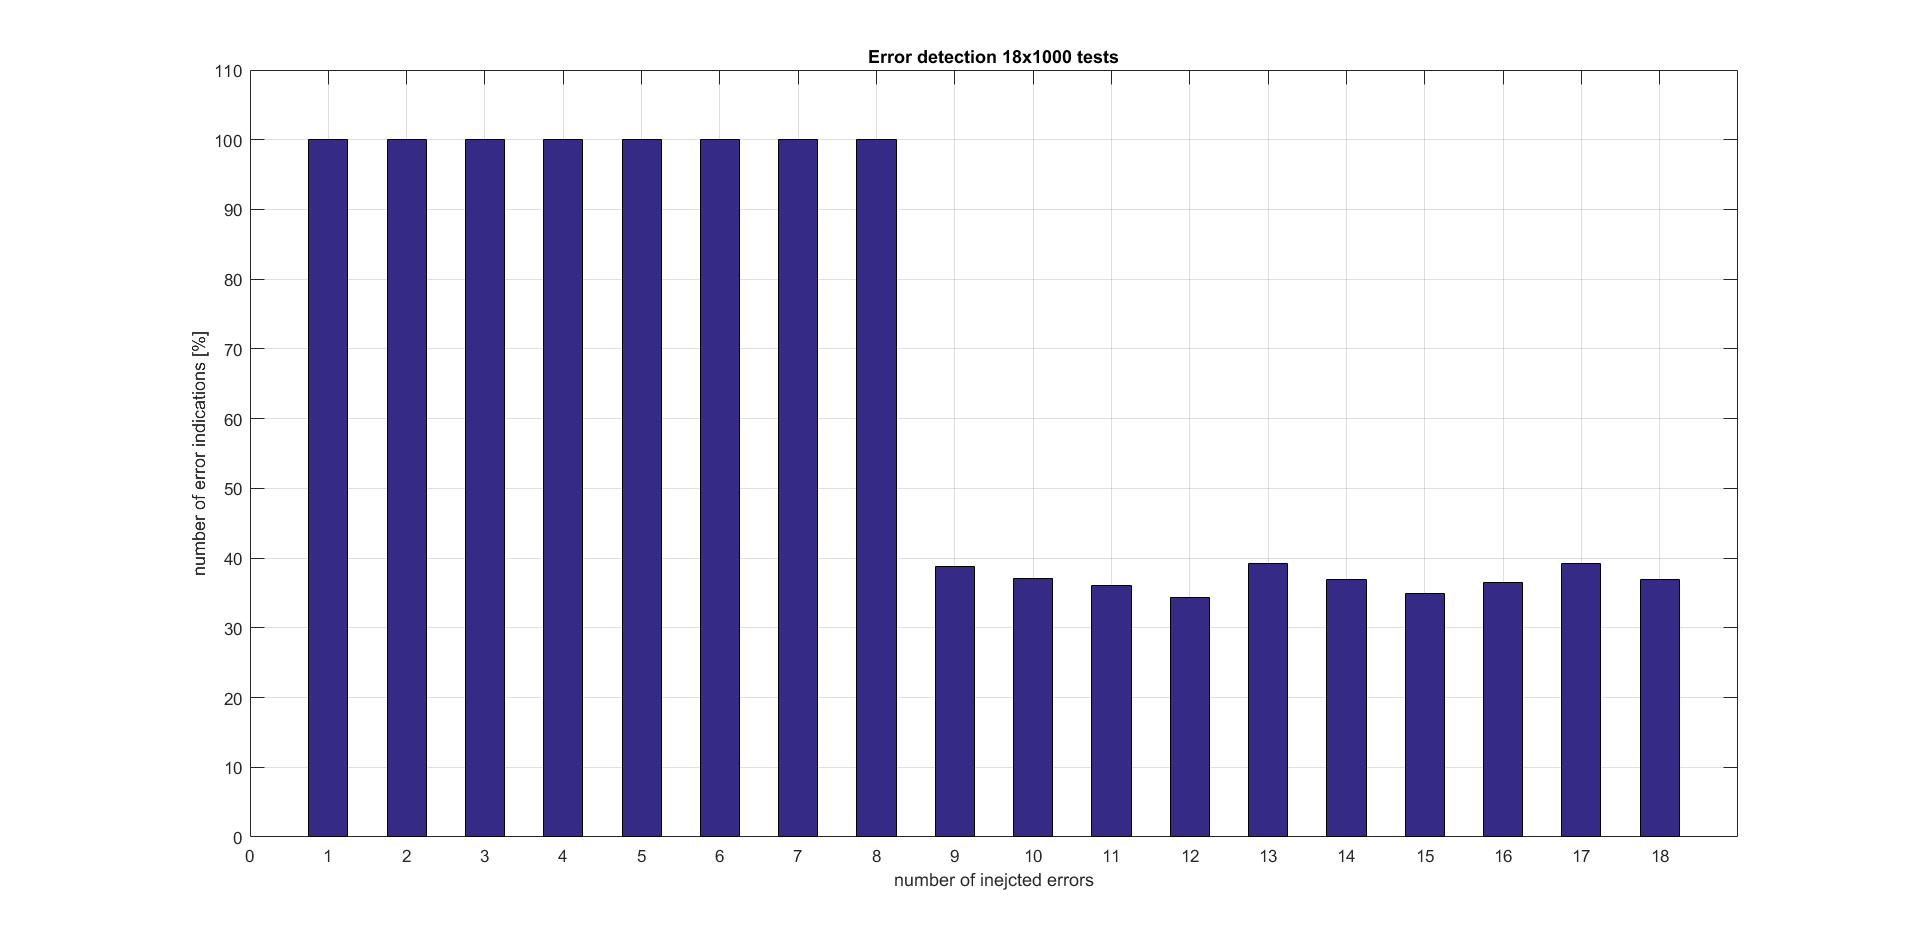
\includegraphics[width=\textwidth]{figures/1000_tests_error_detection.png}
\caption{The error detection limits of the decoder}
\label{fig:dec_1}
\end{figure}

Because the Test Engine allows tests with higher frequencies and the cut-off frequency of the decoder is known to be 229 MHz, the decoder was tested at 230 MHz for its maximal error detection. The result is shown in \autoref{fig:dec_230}

\begin{figure}[h]
\centering
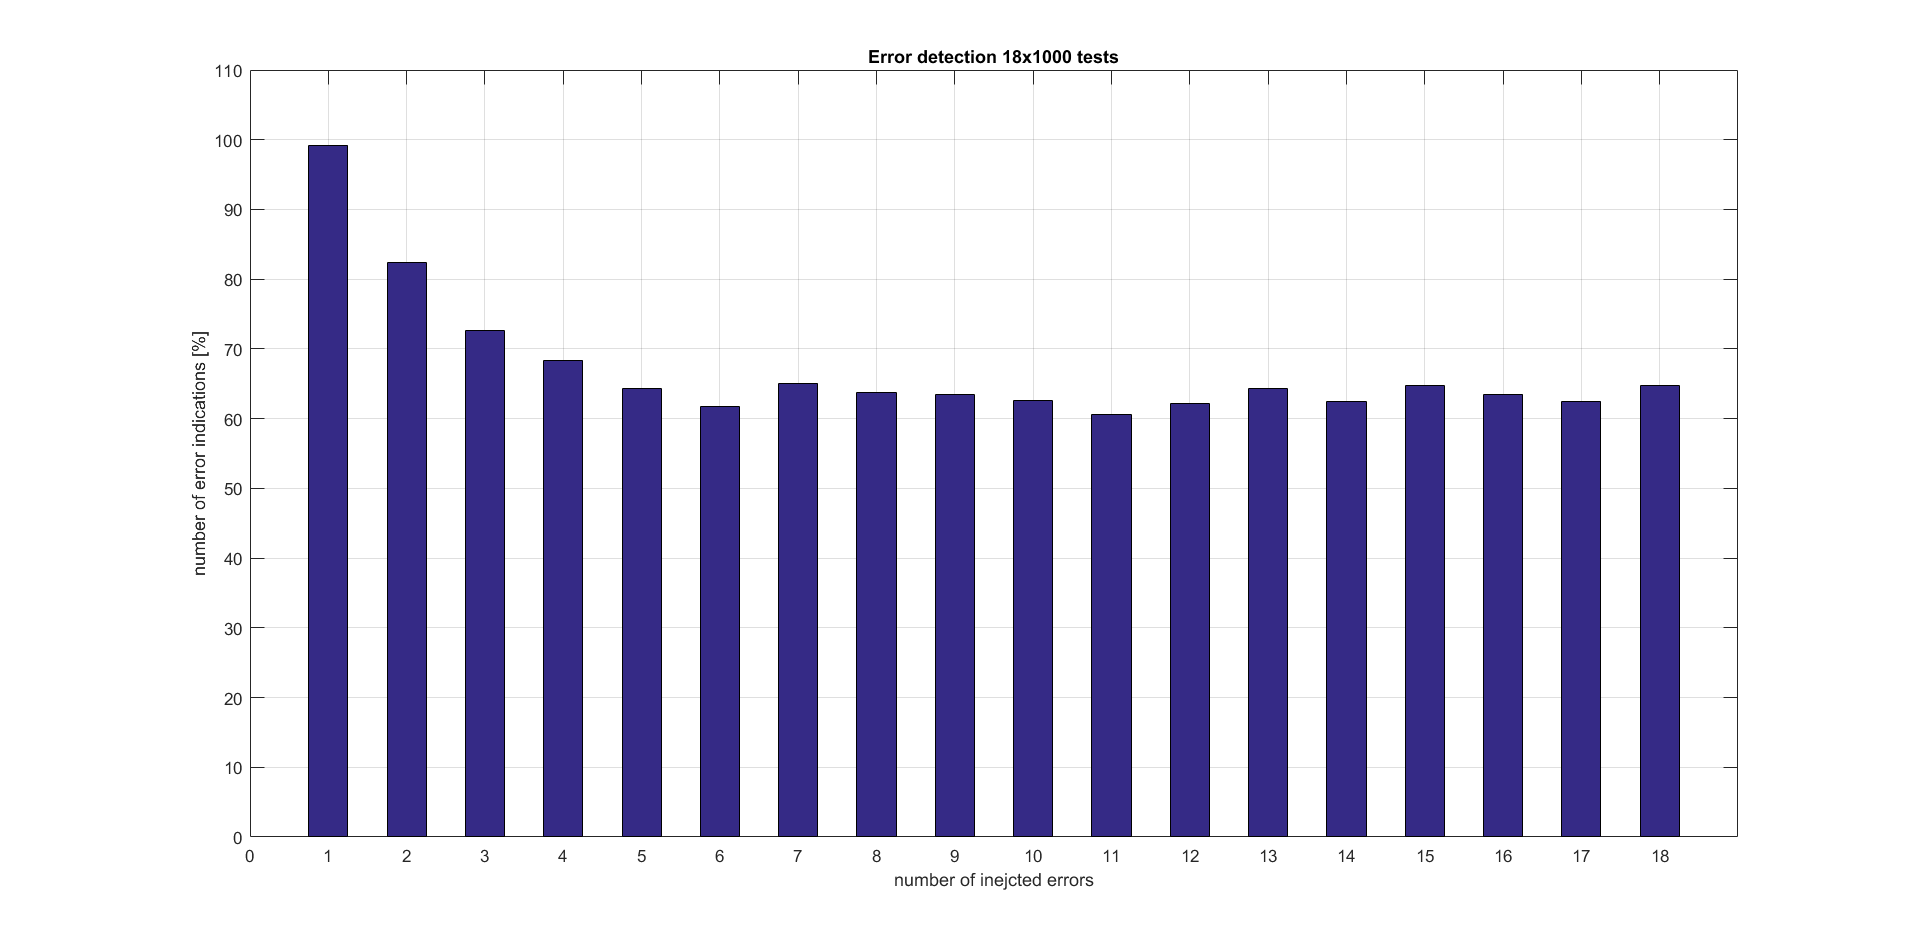
\includegraphics[width=\textwidth]{figures/max_detection_230.png}
\caption{The error detection limits of the decoder at 230 MHz}
\label{fig:dec_1}
\end{figure}

The error detection capability of the decoder was diminished by delay faults happening at 230 MHz. It fails to reliably correct any number of errors, having a 99\% detection rate of single bit errors and 82\% for double bit errors.

The XML file returned by the test engine allows to examine the failed tests and see where the errors occur and in what number. The result evaluation of the test with 1 induced error is showed in \autoref{fig:dec_3}. There are 1000 messages to be corrected and the frequency is just above the limit, tacting the design with 238 MHz. The right-hand side graph shows the total number of errors resulting from overtacting. Their colors correspond to the type of output. They should be equal at all times, since the only way to flip the DOUT bit should be through the ISERR bit. The left-hand side graph represents all erroneous messages and the positions of errors. Dots represent the errors in the DOUT signal, the rectangles - errors in ISERR signal. The diamonds symbolize the positions of injected errors.


\begin{figure}[h]
\centering
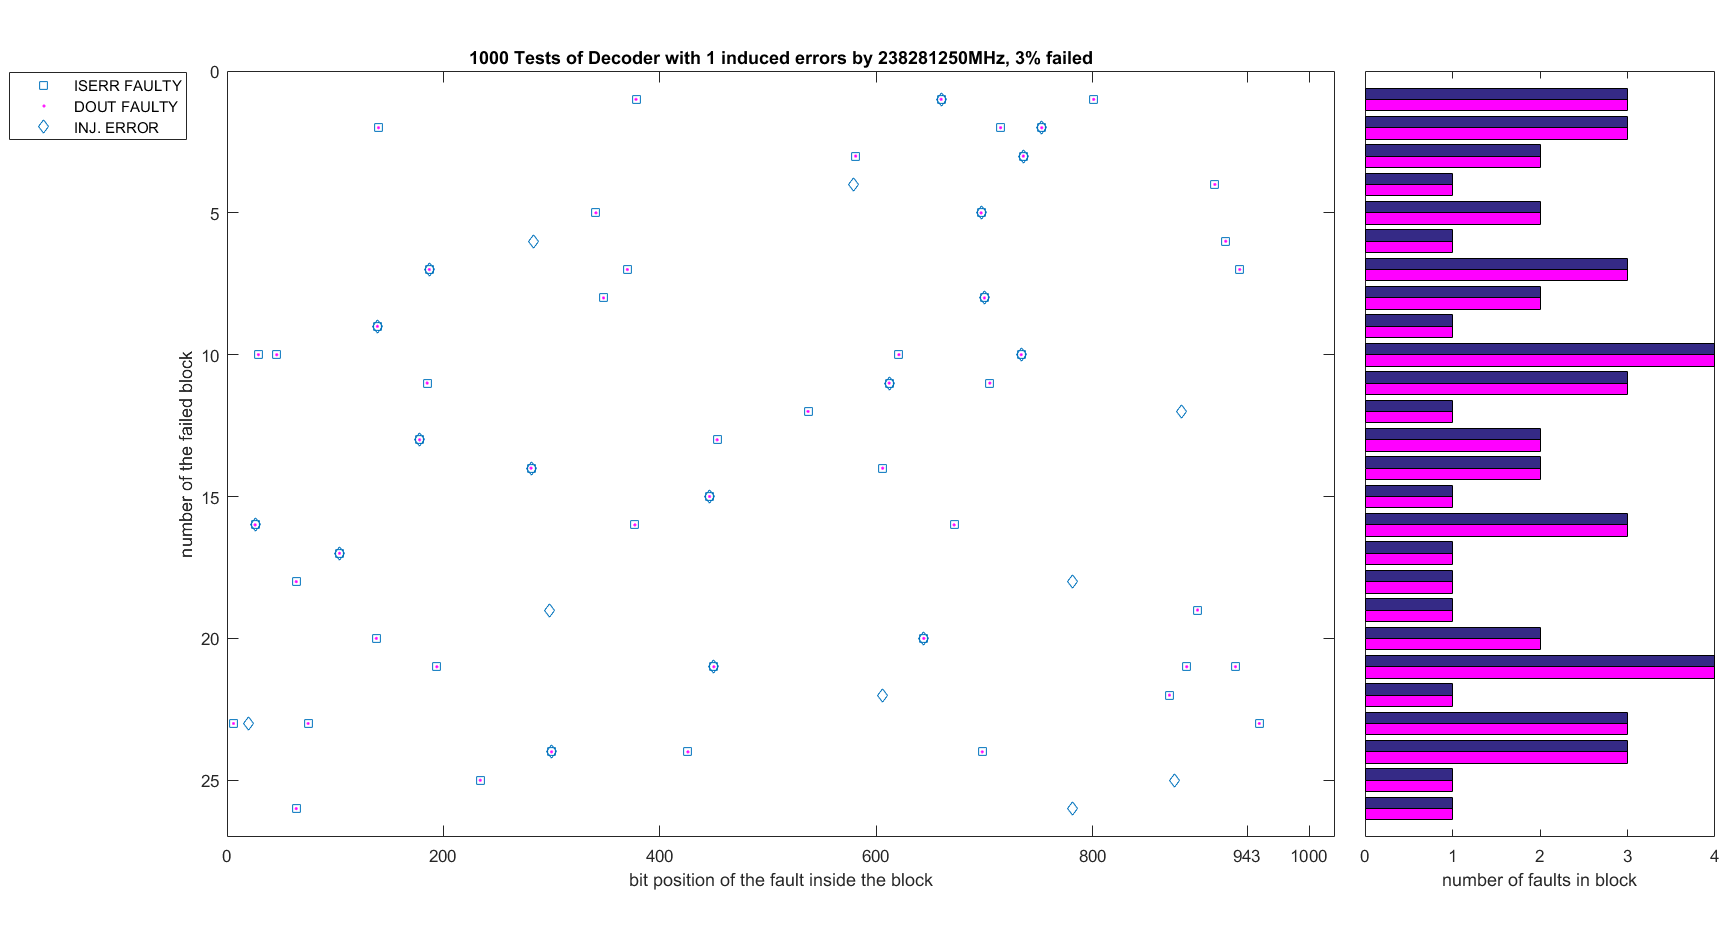
\includegraphics[width=\textwidth]{figures/1000_tests_1_faults_238_MHz.png}
\caption{Test of BCH Decoder with 1 injected error over its max. frequency}
\label{fig:dec_3}
\end{figure}

When the diamond marker is present without other markers it means, that the error was injected in this position and it was detected and corrected successfully. There are two types of errors. When all three markers reside in one position it means, that there was an error injected in this position and it was expected to be detected and corrected. The detection did not happen, therefore it was not corrected, causing an error both in ISERR and DOUT. All other cases are errors that got wrongly detected and corrected although none were injected in those positions - errors induced by decoder itself, marked as rectangle with dot. 

The error distribution is random, data dependent. The single syndrome computation is very similar to the parity computation in the encoder, since it also involves LFSR. The encoder test revealed, that it doesn't fail at such low frequency, hence the errors are produced somewhere in the Key Solver or Chien Search Block. If the Chien Search Block failed, it could produce more errors, then the theoretical decoder correction capability. Such thing was not visible during any of the tests. The fault is therefore probably in the Key Solver or control logic.

\begin{figure}[h]
\centering
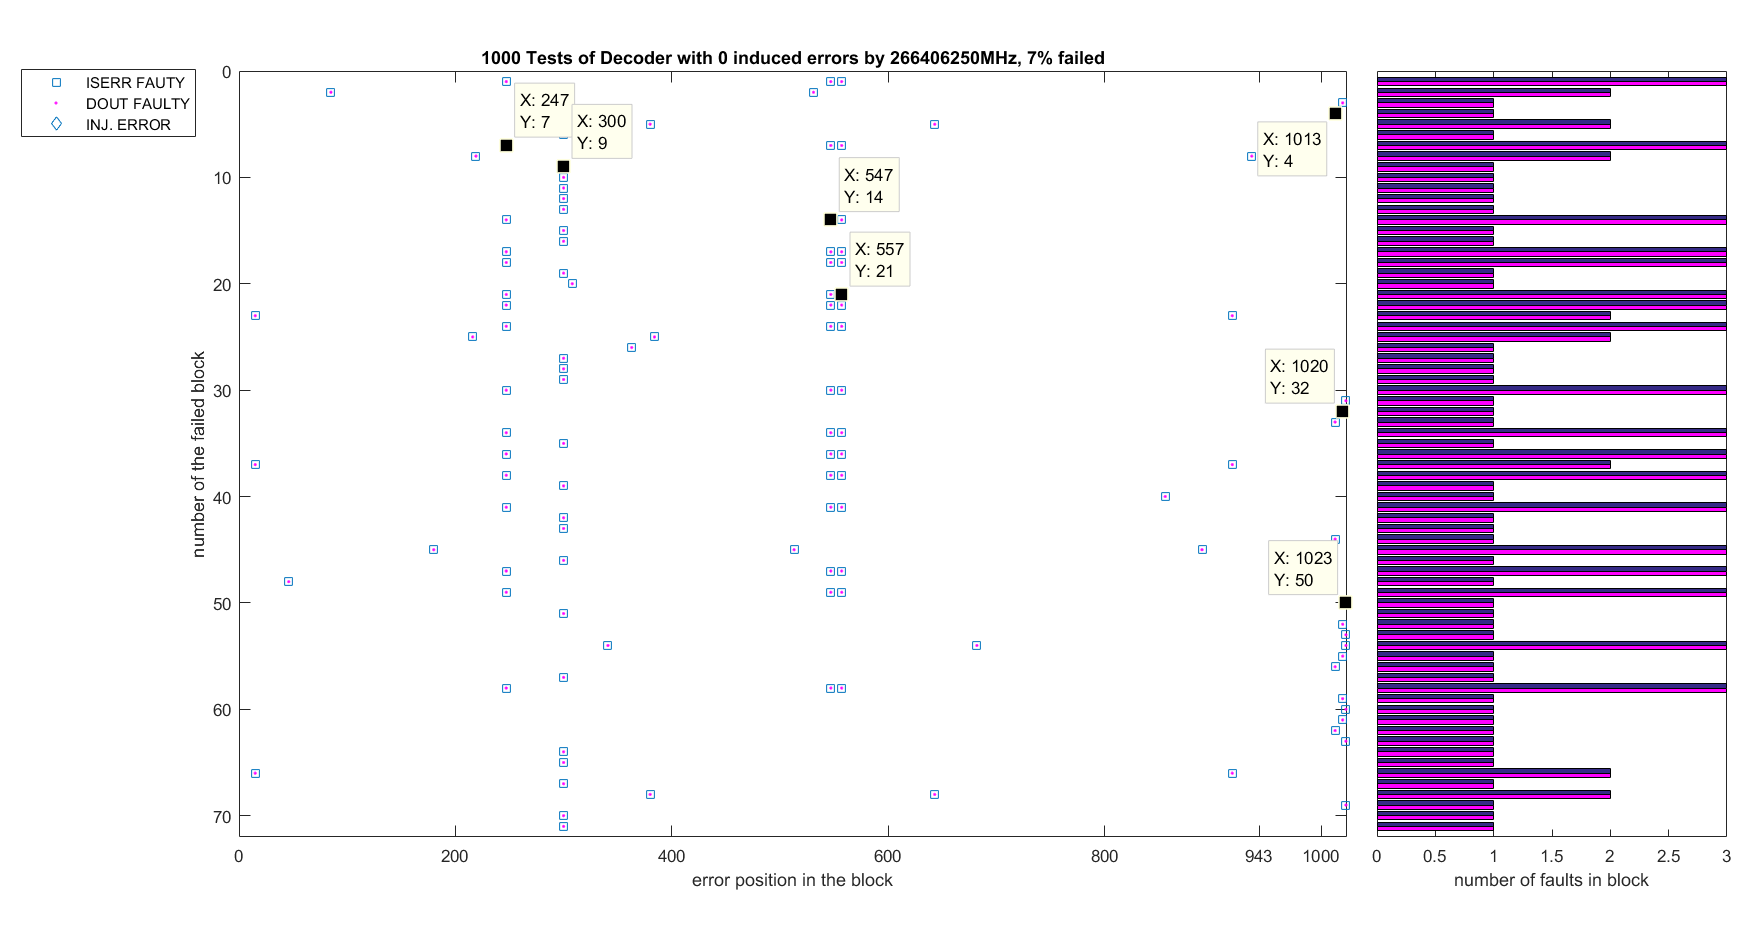
\includegraphics[width=\textwidth]{figures/1000_tests_0_faults_266_MHz_1.png}
\caption{Test of BCH Decoder with 0 injected errors over its max. frequency}
\label{fig:dec_2}
\end{figure}

In the test with no injected errors (\autoref{fig:dec_2}), the syndromes and therefore the parameters of error locator polynomial should be zero at all times. The error positions are not any more data dependent and random, but they occupy mostly the same positions throughout all failed tests. Again the suspected module is the Key Solver.

When the frequency gets closer to 300 MHz another characteristic errors appear in the decoder architecture. At first the result, analyzed as all others, showed a failure of almost all DOUT bits. The plot of this result represents no information at all. In the raw data, it was but visible, that the response signals are somewhat shifted in relation to the expected values. Again a cross-correlation function came to aid and allowed to determine the shift, which is equal $2$. The received signal needs to be shifted by $-2$ (2 to the left) to be aligned with expected signal. The result of the comparison after the shift is shown in \autoref{fig:dec_4}. 

\begin{figure}[h]
\centering
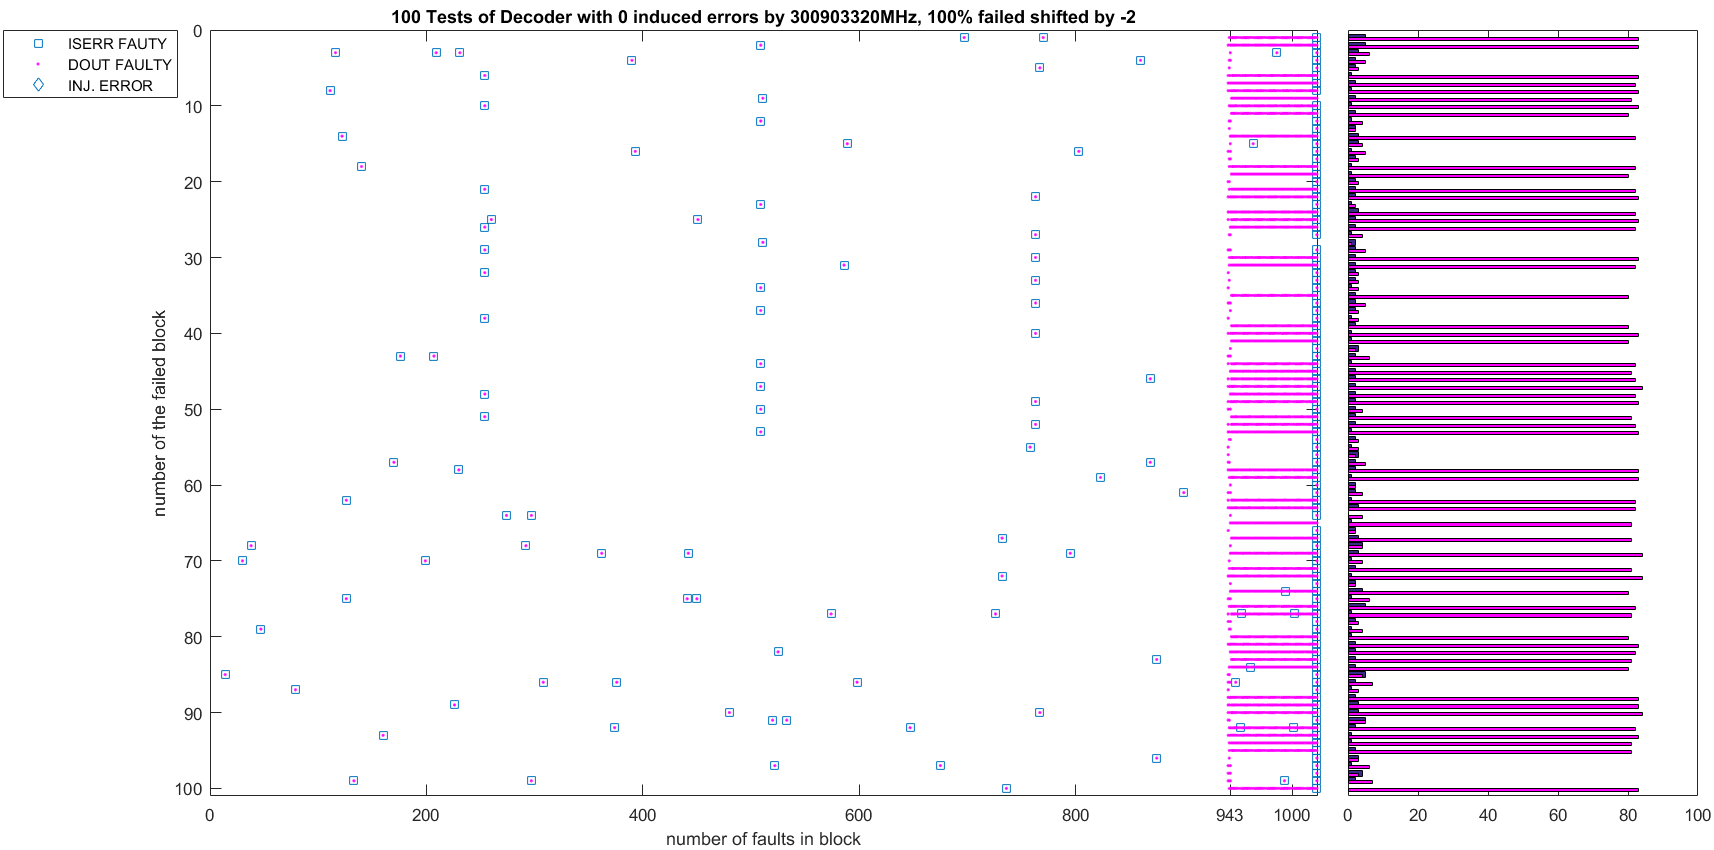
\includegraphics[width=\textwidth]{figures/100_tests_0_faults_300_MHz_shift_2.png}
\caption{Test of BCH Decoder with 0 injected error much over its max. frequency}
\label{fig:dec_4}
\end{figure}

The number of $ISERR$ errors is different then the number of $DOUT$ errors, which means that the error correction logic is not responsible for the wrong output. The further inspection reveals, that the value of 940th data bit (which is still a payload bit) is the last correctly returned value. All following bits are stuck at the value of the 940th input bit. The relation is shown in the \autoref{fig:shift}.

\begin{figure}[h]
\centering
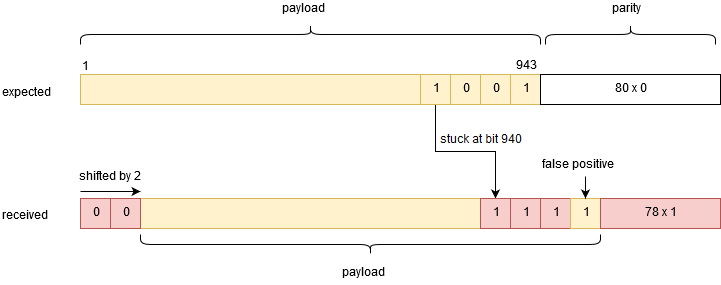
\includegraphics[width=0.65\textwidth]{figures/decoder_parity.png}
\caption{Response shift in the BCH Decoder tested much over it's max. frequency}
\label{fig:shift}
\end{figure}

In the normal operation the parity bits would be 0 and flipped only by Chien Search Block in case of error correction. Since the input data is manipulated only by one logic gate (LUT) during the correction and the $ISERR$ bit is not causing the correction, the error happens in the decoder interface. The design is isolated with additional flip-flops and direct output is always compared with the delayed output to detect the delay errors on the DOUT signal. The same applies for input signal. T

In conclusion, the errors showing up by 300 MHz are due to long paths between the decoder and the test engine, having nothing to do with the internal structure of the decoder.

Failing interconnects lead to interesting conclusion, that the delay faults in the FPGA may be injected by exploiting the placing tools by positioning chosen cells apart from the main design, to guarantee that they will fail as first, when the frequency gets raised. It is important to remind, that the delay faults in real hardware may happen in other paths, not necessarily the longest ones.

 The positions of errors did not change, only the frequency, when they started to appear. The delay fault on the interconnect doesn't appear until 365 MHz. This time the delay faults were detected thanks to the delay logic.

The placement of the design seems to have great impact on test results. The delay faults happening on the interface can be detected by delay logic and comparison, but the placement of this logic is also of grave importance. The decoder circuit is unable to detect more errors then it can correct. In case of permanent faults in the decoder, special BIST techniques need to be incorporated, since the faults will have influence on the results of the diagnostic test. The diagnostic test can show that the decoder or encoder is faulty. Since the encoder faults are expected to produce errors in parity bits and the decoder errors reside randomly in the whole code word, the position of the error should give good indication on which module failed. The additional internal test can be conducted with suggested method of testing the LFSRs \cite{art:Gleichner} or in regular decoder circuits, like Hsiao-Code decoders, using spare modules and glitch filters \cite{art:Dicorato}.


\chapter{Summary}

The diagnostic test is limited by the error detection capability of the decoder. The more errors a decoder can detect, the better chance of reliable test result. In systems with single error correction and double error detection (SEC-DEC), like those implementing extended Hamming-code or Hsiao-code, the common weak point is erroneous error detection in case of triple bit errors and multiple bit errors \cite{art:Dicorato}. The diagnostic test based on those modules may produce false positive results in such systems, assuming that single fault may corrupt more bits in the data bit stream. In communication systems, where data is processed serially, like in BCH encoder and decoder tested in this thesis, the occurrence of multiple bit flips in case of single fault is very high. In case of BCH decoders, it may require to redesign the architecture to implement the capabilities of underlaying ECC fully or in case of PENCA, which is a reconfigurable solution, to choose the code with highest correction capability, which is 15 bit errors in a single message \cite{art:Pfeifer}.

Another limitation to the diagnostic test solution is the coverage of only those modules, which lay between encoder and decoder. The source encoding and cryptographic encryption are only two examples of modules, that may reside outside of the test subsystem, not covered by the diagnostic test. For those modules, well established digital test methods need to be applied. The same restriction applies to the decoder architecture itself. It has been admittedly reported, that some decoder architectures, like Hsiao-code decoder are capable of correcting (masking) some of its own hardware faults happening in the embedded encoder structure, under condition that they don't overlap with the transmission errors \cite{art:Dicorato}, but this feature does not cover the entire decoder structure and lowers the error coverage of the deocder. In the BCH decoder if any syndrome is non-zero a correction is triggered, so any fault in syndrome generation unit, that leads to a failure of the unit, will trigger a false correction, therefore an error in output bit stream. The same applies to the Key Solver unit or Chien Search Block. In all cases, the diagnostic test doesn't cover the decoder internal faults so the decoder dependability needs to be taken care of separately. The diagnostic test can help in finding encoder or decoder faulty, since the last shortcut tests only those two modules. In case of failed test, as in all other cases, the repair of one unit is conducted and the test is repeated.

Moreover the diagnostic test is used only for error detection. The repair of permanent faults require further redundancy, like spare units, leading to duplication of the hardware or parts of it. In case of patent protected circuitry, with no additional DfT extensions, a full duplication of hardware seems to be the only way to ensure repair possibility. Thanks to the diagnostic test, there is no need for trippling the hardware to create a TMR system.

The additional multiplexers, laying on transmission path, lead to signal deterioration, which is especially important in the analog part. The multiplexers need to be adjusted, so that their response does not disturb "normal" functionality of the system. In digital logic, the additional multiplexers create additional delay, although the switching happens off-line, so it should not influence the "normal" function.

The suggested diagnostic test requires also control logic to conduct the "fake" start-up procedure and maybe run some additional test vectors through the design to detect faults not visible during the start-up phase. Most of it can reside in software, since the test uses "normal" data path. The only signals needed during the implementation were the $ISERR$ output of the decoder and control signals to enable shortcuts. To conduct the repair, additional control inputs need to be provided.

In conclusion, the suggested solution is useful as diagnostic test in systems with no internal access to some modules laying between FEC encoder and decoder and allows the test of analog, mixed-signal and digital modules indifferently with just little hardware and software overhead. The test is limited by error detection capability of the decoder. The limitation is not different then the test result evaluation using signatures. The tests are false positive in case of error vectors changing one code word into another valid code word, just like conflicts happening in signature calculation. To extend the test to all modules in transceiver and receiver, more shortcuts can be added, between all corresponding modules, and the response analysis may happen in the software. This approach may be triggered when the proposed diagnostic test fails its purpose.

The results of tests conducted on encoder and decoder architectures, helped by the development process and were a valuable input in understanding the limitations of the designs. They also validated the proper functionality of the basic PENCA building blocks and showed, in case of decoder, where are the possible bottlenecks. Unfortunately, the test engine was not successful in testing the limits of encoder architecture.

As a result of this thesis, a useful tool for design validation in "real" hardware was developed and may be used as an alternative to simulation, speeding up the development process and allowing quick evaluation of responses with any chosen program. The placement of the design is to be treated with much caution and understanding, to avoid misinterpretation of test results. 